% Bachelor Degree Thesis - Paolo Lucchesi
% !TeX encoding = UTF-8
% !TeX program = pdflatex
% !TeX spellcheck = en_US

\documentclass[binding=0.6cm,Lau]{sapthesis}
\usepackage{microtype}
\usepackage[english]{babel}
\usepackage[utf8]{inputenc}
\usepackage{hyperref}
\usepackage{tabularx}
\usepackage{fontspec}
\usepackage{setspace}

\setmainfont{TeX Gyre Pagella}
\onehalfspacing


\makeatletter
\def\maxwidth#1{\ifdim\Gin@nat@width>#1 #1\else\Gin@nat@width\fi}
\makeatother

\hypersetup{pdftitle={AVR Multi Motor Control},pdfauthor={Paolo Lucchesi}}

\title{AVR Multi Motor Control}
\author{Paolo Lucchesi}
\IDnumber{1765134}
\course{Ingegneria Informatica e Automatica}
\courseorganizer{Facoltà di Ingegneria dell'Informazione, Informatica e Statistica}
\AcademicYear{2021/2022}
\copyyear{2021}
\advisor{Prof. Giorgio Grisetti}
\advisor{Drs. Barbara Bazzana}
\reviewerlabel{Reviewer}
\reviewer{Prof. Silvia Bonomi}
\authoremail{lucchesi.1765134@studenti.uniroma1.it}
\website{https://github.com/jcondor98/ammc}


\begin{document}

\frontmatter
\maketitle

\dedication{
Dedicated to my family, my granddad Pietro, my mom Anna Rosa, my dad Marco,
my grandmom Pierina and my sister Valentina, which I thank everyday for
everything I am.\\
To my dearest friends in Pitigliano, with whom I share some of the most
beautiful memories I have.\\
To Nicola, with whom I have shared part of this path; he helped me in a
dark period of my life and he is one of my dearest friends.
}

\begin{abstract}
  Nowadays, men physical work is gradually being taken or eased by technology.
  Many solutions in this area of interest rely on the use of electrical motors
  to accomplish tasks. Furthermore, electrical motors are widely used in many
  retail products, such as toys, domotic devices and so on.

  In this work I propose, as the result of my bachelor degree apprenticeship,
  the \emph{AVR Multi Motor Control} ecosystem as a solution for the management
  of multiple dc motors. It is composed of a client application for user
  interaction, a \emph{master} controller and multiple slave controllers, each
  handling a single motor. The master controller manages slave controllers,
  reading and manipulating the dc motors' speed with granularity.

  In chapter \ref{ch:intro} I give a broad overview on the work done, focusing
  on the structure of the entire project and the approach I had relating to 
  software architecture, coding and documentation writing.

  In chapter \ref{ch:client} I discuss the client-side application, focusing on
  user interaction and software architectural characteristics.

  In chapter \ref{ch:master} I discuss the master controller, focusing on
  hardware setup and firmware internals.

  In chapter \ref{ch:slave} I discuss the slave controller, focusing on
  hardware and the software-defined Proportional-Integral-Derivative controller
  embedded in the firmware.

  In chapter \ref{ch:client-master-comm} I discuss the protocols responsible
  for the communication between the client application and the master
  controller, and how I used the underlying serial communication channel.

  In chapter \ref{ch:master-slave-comm} I explain how I used the I2C bus to
  connect the master controller to multiple slave controllers.
\end{abstract}

\tableofcontents
\listoffigures
\listoftables

\mainmatter

\chapter{Introduction}
\label{ch:intro}

\section{Motivation}
The use of dc motors is widespread in many application fields. Often, the
offered solutions are monolithic and use of very specific (and sometimes ad-hoc
developed) hardware. The ammc ecosystem focuses on the use of very common,
affordable and easily available hardware, such as AVR microcontrollers.

The software is designed to be modular, extensible and easily hackable by any
average C programmer, so that in the future other people interested in this
project can contribute or adapt ammc to fit their needings and accomplish their
business logic.

\section{Contributions}
The ammc ecosystem offers a flexible, affordable, hackable solution for the
management of multiple dc motors. It is composed of three main components:

\begin{itemize}
  \item A client-side application
  \item A master controller
  \item One or more slave controllers
\end{itemize}

\subsection{Client}
The client-side application is written in C. It makes use of the POSIX standard
library, and in particular the \emph{termios} interface to generic serial
devices. It offers a shell-fashioned terminal user interface.

\subsection{Master}
The master controller is an AVR microcontroller unit. The firmware is written
in C, using the \emph{avr-gcc} compiler and the \emph{avr-libc} standard
library implementation. It dispatches user commands (taken by the client) to
slave controllers.

\subsection{Slave}
The slave controllers are AVR microcontroller units. The firmware is written in
C, using the \emph{avr-gcc} compiler and the \emph{avr-libc} standard library
implementation. Each slave controller manages a single dc motor, taking
commands by the master controller.

\section{Technical approach}

\subsection{Software architecture}
I have developed all the top-level ammc components following the principles I
have learned both from my University courses\cite{fondamenti2-prog} and my
personal insights\cite{clean-architecture}\cite{cpp-ref}.

The client application and the microcontroller firmwares were developed
following the \emph{SOLID} principles, with attention on the \emph{Open-Close
principle}.  I have put particular attention on modularity; many of the
software modules found in all the ammc applications are standalone and will
work out of the box if brought into other projects.

I tried to develop my software with the following policy: the core of the
application should be composed of reusable, standalone modules; the business
logic of the application, which obviously changes radically from project to
project, should be placed in the peripheral modules and should use, when
possible, interfaces for dependency inversion towards the core modules.

For example, in the master controller firmware source code I use function
pointers to generalize the operations to be triggered by client commands.
Naturally, such practices would have been easier and more evident with a
programming language explicitly supporting the object-oriented paradigm (e.g.\
C++).

\subsection{Documentation}
Documentation is paramount in any software project; Damian Conway once said:
"Documentation is a love letter that you write to your future self". I did my
best to write precise and exhaustive documentation for every software piece I
realized.

This thesis is by itself a document dealing with every aspect of the ammc
project. The \texttt{README.md} file in the root directory of the repository
offers a more concise resume.

All the source code (the head files in particular) are exhaustively documented
with \emph{doxygen}, a tool which automatically converts properly formatted
comments found in the code into technical documentation; such resource is
available in the \texttt{gh-pages} git development branch and is hosted using
GitHub Pages.

The client-side application is documented with a Unix man page, which can also
be found in this thesis in section \ref{sec:client-manpage}.


\chapter{Client-side user interaction}
\label{ch:client}
A client program has been realized to manipulate the dc motors directly from the
PC. It can get and set the speed of individual motors, and to apply all the
previously set speeds for all of them at once.\\ A brief list of the
client's features is given below:
\begin{itemize}
  \item Granular handling for getting and setting motors' speed
  \item Modular and extensible software architecture
  \item Terminal User Interface, implemented as a command shell
  \item Support for non-interactive use (i.e.\ scripting)
  \item Communication with master controller using the serial protocol
  \item Compatible with POSIX-compliant environments
\end{itemize}
The client is also documented with a man page, which can be found in section
\ref{sec:client-manpage}.

\section{User Interface}
The end user interacts with the whole ammc ecosystem using a text-based client.
It consists in a shell module, which I had written myself, offering some
\emph{internal commands} (hardcoded in the shell module itself) and is extended
by \emph{external commands} (found in a separated source code entity, and that
can even be compiled in a detached transaction unit).

A particular focus was made on the software architecture: indeed, every
external command can be realized standalone, and it is easy to add new
commands just by altering the \texttt{client/source/shell\_commands.c} source
file.

\section{Primitives offered}
The commands that can be used to interface with the ammc ecosystem are the
following:
\begin{description}
  \item[connect <device-path>] Connect to a master controller, given the path
    to the block device representing it.
  \item[get-speed <motor-id>] Get the speed of a dc motor given its id.
    The motor id must be specified as a decimal number.
  \item[set-speed <motor-id>=<speed>] Set the speed of a dc motor given its id.
    The motor id must be specified as a decimal number and the speed must be
    specified in rpm.
  \item[apply] Apply the previously set speed for all the dc motors.
\end{description}

\subsection{Non-interactive mode}
The client shell is capable of running in non-interactive (i.e.\ scripting)
mode with the \texttt{-s} option.  If so, it will parse the input from a
specified text file, or from \texttt{stdin} if not provided.  A shell launched
in non-interactive mode will not print shell prompts, and exit when end-of-file
is encountered or on command failure.

\section{Serial module}
The client's serial module has been realized using the POSIX \emph{termios}
interface. Unlike the master controller's counterpart, all its code is
reentrant, therefore multiple instances of multiple serial devices can
theoretically exist at the same time.

From the client's perspective, the master controller is seen as a file
descriptor, and the end user just have to specify the path of the block device
file representing the serial communication channel (e.g. \texttt{/dev/ttyACM0})
using the \texttt{connect} command.

\section{Specification}

\subsection{Software modules}
An exhaustive list of software modules for the client application is given
in table \ref{tab:client-spec-modules}. File paths are relative to the
\texttt{client/} directory.

\begin{table}[bh]
  \begin{tabularx}{\textwidth}{c X X}
    \toprule
    Module & Description & Files \\
    \midrule
    communication &
      Contains all the top-level communication routines &
      \texttt{include/communication.h}, \texttt{source/communication.c} \\
    crc &
      Contains the CRC generation and checking routines &
      \texttt{include/crc.h}, \texttt{source/crc.c} \\
    debug &
      Contains convenient debug facilities &
      \texttt{include/debug.h} \\
    main &
      Contains the main client application routine &
      \texttt{source/main.c} \\
    packet &
      Contains packet generation and manipulation routines &
      \texttt{include/packet.h}, \texttt{source/packet.c} \\
    ringbuffer &
      Circular buffer implementation for the serial module &
      \texttt{include/ringbuffer.h}, \texttt{source/ringbuffer.c} \\
    serial &
      Contains all the routines for the underlying serial communication layer &
      \texttt{include/serial.h}, \texttt{source/serial.c} \\
    shell &
      Main program shell with built-in commands &
      \texttt{include/shell.h}, \texttt{source/shell.c} \\
    shell\_commands &
      Contains the custom external commands to interact with the master controller &
      \texttt{source/shell\_commands.c} \\
    \bottomrule
  \end{tabularx}
  \caption{Client application software modules}
  \label{tab:client-spec-modules}
\end{table}

\subsection{Modules dependency graph}
The dependency graph for the client application software modules is shown in
figure \ref{img:client-deps-graph}. The \emph{debug} module is excluded. Notice
how the dependency flow goes in one direction (from top to bottom); this is the
result of the software architecture policy used.
\begin{figure}[hbp]
\begin{centering}
  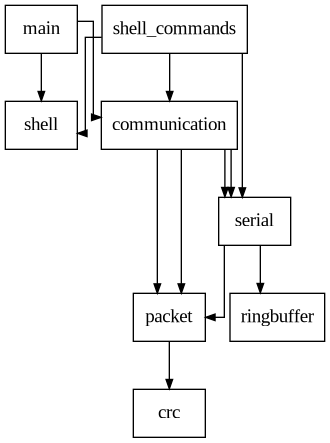
\includegraphics[scale=0.5]{img/client-deps}
  \caption{Client application modules dependency graph}
  \label{img:client-deps-graph}
\end{centering}
\end{figure}

\section{Man page}
\label{sec:client-manpage}


\chapter{Master controller}
\label{ch:master}
The master controller handles all the slave controllers, dispaching arbitrary
commands to them using the I2C protocol. It also communicates directly with the
client application via serial port.

\section{Hardware setup}
The master controller itself is an AVR \emph{ATMega2560} microcontroller
unit\cite{at2560-ref}. This particular MCU has features convenient for this
project, such as:
\begin{itemize}
  \item I2C dedicated hardware subsystem
  \item Serial-over-USB bridge
  \item Relatively powerful specifications for future feature adding
  \item Plenty of timers and outgoing power pins
\end{itemize}

A $100 pF$ capacitor is used to block the reset capabilities of the
serial-over-usb controller and enhance the serial channel reliability. Two
$4.7 k\Omega$ resistors are used as open-drain resistors for the I2C bus.

\section{I2C setup}
The I2C protocol is used to communicate with slave controllers. Transmission
and reception are interrupt-based, and no busy-wait is used.

The I2C module has broadcasting capabilities, according to the informations
found in the I2C standard I2C standard\cite{i2c-ref}; the broadcasting (i.e.\
\emph{general call}) address used is \texttt{0x00}. As stated by the standard,
the master controller has no knowledge on the number or identity of the slaves
receiving a broadcast frame.

\section{Power management}
An own-written wrapper for the avr-gcc standard library's sleep functionalities
is used for power management.  By default, the master controller is in
\emph{idle} mode, and it is awakened by any raised interrupt, e.g.\ by incoming
serial or I2C data; then, its main loop routine is executed and, if no other
operations must be performed, it returns in idle mode.

The master controller is also put in idle when waiting for data inside serial
or I2C routines; this is possible thanks to the interrupt-driven nature of the
aforementioned modules.

\section{Specification}

\subsection{Software modules}
An exhaustive list of software modules for the master controller firmware is
given in table \ref{tab:master-spec-modules}. File paths are relative to the
\texttt{master/} directory.

\begin{table}[bh]
  \begin{tabularx}{\textwidth}{c X X}
    \toprule
    Module & Description & Files \\
    \midrule
    communication &
      Contains all the top-level communication routines &
      \texttt{include/communication.h}, \texttt{source/communication.c} \\
    crc &
      Contains the CRC generation and checking routines &
      \texttt{include/crc.h}, \texttt{source/crc.c} \\
    dcmotor &
      Contains the top-level routines for interfacing slave controllers &
      \texttt{include/dcmotor.h}, \texttt{source/dcmotor.c} \\
    main &
      Contains the main and power management routines &
      \texttt{source/main.c} \\
    packet &
      Contains packet generation and manipulation routines &
      \texttt{include/packet.h}, \texttt{source/packet.c} \\
    ringbuffer &
      Circular buffer implementation for the serial module &
      \texttt{include/ringbuffer.h}, \texttt{source/ringbuffer.c} \\
    serial &
      Contains all the routines for the underlying serial communication layer &
      \texttt{include/serial.h}, \texttt{source/serial.c} \\
    sleep\_util &
      Handy wrapper for the avr-libc power management facilities &
      \texttt{include/sleep\_util.h} \\
    twi &
      Contains the I2C/TWI layer which underlies the communication between master and slaves &
      \texttt{include/twi.h}, \texttt{source/twi.c} \\
    \bottomrule
  \end{tabularx}
  \caption{Master application software modules}
  \label{tab:master-spec-modules}
\end{table}

\subsection{Modules dependency graph}
The dependency graph for the master controller's software modules is shown in
figure \ref{img:master-deps-graph}. The \emph{debug} module is excluded. Notice
how the dependency flow goes in one direction (from top to bottom); this is the
result of the software architecture policy used.
\begin{figure}[hbp]
\begin{centering}
  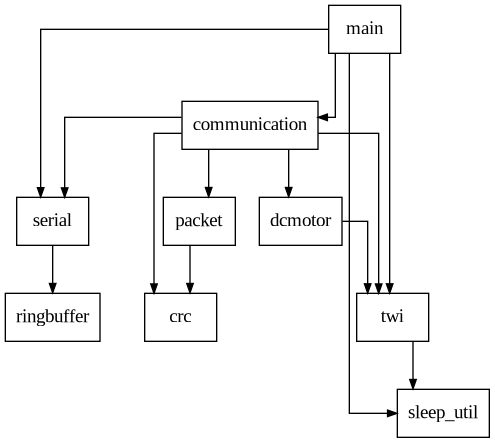
\includegraphics[scale=0.5]{img/master-deps}
  \caption{Master controller modules dependency graph}
  \label{img:master-deps-graph}
\end{centering}
\end{figure}

\subsection{Circuit schematics}
The complete circuit schematics for the master controller and all its components
is shown in figure \ref{img:master-sch}.
\begin{figure}[hbp]
\begin{centering}
  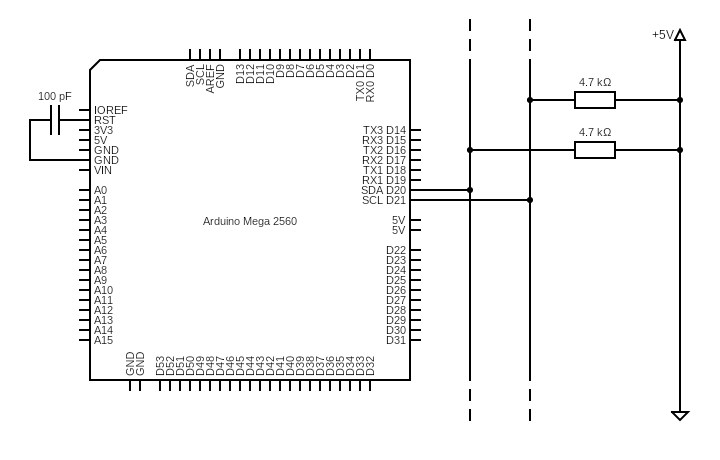
\includegraphics[width=\maxwidth{\textwidth}]{img/master-schematics}
  \caption{Master controller schematics}
  \label{img:master-sch}
\end{centering}
\end{figure}

\subsection{Wiring}
The wiring correspondence for the master controller MCU is shown in table
\ref{tab:master-wiring}.
\begin{table}[hb]
  \begin{tabularx}{\textwidth}{c l X}
    \toprule
    Board pin & MCU pin & Description \\
    \midrule
    D20 & 44/PD1/INT1/SDA  & I2C data bus \\
    D21 & 43/PD0/INT0/SCL  & I2C clock bus \\
    RESET & RESET & On-board MCU reset pin \\
    \bottomrule
  \end{tabularx}
  \caption{Master controller wiring}
  \label{tab:master-wiring}
\end{table}



\chapter{Slave controllers}
\label{ch:slave}
Each slave controller directly handles a single dc motor, receiving commands
from the master controller via I2C. It must offer an interface to get and
manipulate its motor's speed.

The slave controller produces a PWM wave having a duty cycle consistent with
the speed (given in RPM) specified by the end user in order to control its
motor.

Furthermore, it comes with a software Proportional-Integral-Derivative
controller to correct the bias between target and actual motor speeds.

\section{Hardware setup}
The slave controller itself is an AVR \emph{ATMega328P} microcontroller
unit\cite{at328p-ref}, which offers the following features of interest:

\begin{itemize}
  \item CH340 Serial-over-USB controller for convenient firmware flashing
  \item Reduced size
  \item Relatively high clock and resources
  \item Dedicated I2C hardware subsystem
  \item PWM-capable 8-bit and 16-bit timers
\end{itemize}

Apart from the motor itself (along with its power supply and eventually its
dedicated control board) no additional hardware is used.

\section{I2C setup}
A slave controller communicates with the master controller using the I2C
protocol. As for the master controller, both transmission and reception are
interrupt-based.

The slave controller is always passive on the bus, waiting to be addressed by
the master.

% TODO: Dynamic addressing

\section{Proportional-Integral-Derivative controller}
An own-written, software-defined Proportional-Integral-Derivative controller is
used to correct the actual motor speed. As for any PID device, the equation
controlling the error is:
\begin{equation}
  u(t) = K_p e(t) + K_i \int_{t_0}^t e(\tau)\,d\tau + K_d \frac{d}{dt}\,e(t)
\end{equation}
being:
\begin{itemize}
  \item $u(t)$ the PID control variable
  \item $K_p$ the proportional gain
  \item $K_i$ the integral gain
  \item $K_d$ the derivative gain
  \item $e(t)$ the measured speed error
\end{itemize}

\subsection{Measuring speed}
For actual PID capabilities, the slave controller must sample the actual speed
of the dc motor at fixed intervals. Therefore, the motor must have an embedded,
two-phase digital encoder.

In fact, one phase is wired to an interrupt-enabled input pin, so the slave
controller is notified immediately when an encoder signal (raising edge) is
generated. Every sampling intervals, the PID routine takes the motor's actual
position (measured by the cumulative number of encoder triggers) and computes
its real speed.

\subsection{Approximations}
Of course, a software digital PID controller can not compute exact integrals
and derivatives, so it is necessary to use approximation.

The integral operation is approximated using \emph{Riemann sums}. Given a time
delta $\Delta t$ (the actual speed sampling interval in this particular case),
the approximating law is defined as:
\begin{equation}
  \int_{t_0}^t e(\tau)\,d\tau \approx \sum_{k=1}^n e(t_k^*) \cdot \Delta t
\end{equation}
The derivative operation is approximated using its
definition\cite{levy-num-analysis}:
\begin{equation}
  \frac{d}{dt}\,e(t) = \lim_{\Delta t \to 0} \frac{e(t + \Delta t) - e(t)}{\Delta t} \implies
  \frac{d}{dt}\,e(t) \approx \frac{e(t + \Delta t) - e(t)}{\Delta t}
\end{equation}
being $\Delta t$ a time delta (again, the actual speed sampling interval).

\section{Power management}
The same avr-libc wrapper written for the master controller power management is
used.
By default, the slave controller is in \emph{idle} mode, and it is awakened by
any raised interrupt. The main loop routine is executed and the idle mode is
entered again. Like for the master controller, the slave is put in idle when
waiting for the I2C routines to return.

The AVR idle mode allows the timers to work, so the slave controller can
generate PWM waves to control the motors, even while sleeping.

\section{Specification}

\subsection{Software modules}
An exhaustive list of software modules for the slave controllers firmware is
given in table \ref{tab:slave-spec-modules}. File paths are relative to the
\texttt{slave/} directory.

\begin{table}[bh]
  \begin{tabularx}{\textwidth}{c X X}
    \toprule
    Module & Description & Files \\
    \midrule
    dcmotor &
      Contains stuff to directly manipulate dc motors, including the PID controller, PWM waves generation and speed manipulation routines &
      \texttt{include/dcmotor.h}, \texttt{source/dcmotor.c} \\
    main &
      Contains the main and power management routines &
      \texttt{source/main.c} \\
    sleep\_util &
      Handy wrapper for the avr-libc power management facilities &
      \texttt{include/sleep\_util.h} \\
    twi &
      Contains the I2C/TWI layer which underlies the communication between master and slaves &
      \texttt{include/twi.h}, \texttt{source/twi.c} \\
    \bottomrule
  \end{tabularx}
  \caption{Slave application software modules}
  \label{tab:slave-spec-modules}
\end{table}


\subsection{Modules dependency graph}
The dependency graph for the slave controllers' software modules is shown in
figure \ref{img:slave-deps-graph}. The \emph{debug} module is excluded.
\begin{figure}[hbp]
\begin{centering}
  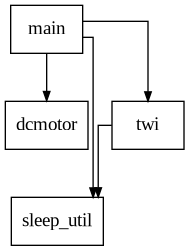
\includegraphics[scale=0.5]{img/slave-deps}
  \caption{Slave controller modules dependency graph}
  \label{img:slave-deps-graph}
\end{centering}
\end{figure}

\subsection{Circuit schematics}
The complete circuit schematics for the slave controller and all its components
is shown in figure \ref{img:slave-sch}. This circuit can be repeated multiple
times (up to 126) in a single ammc ecosystem.
\begin{figure}[hbp]
\begin{centering}
  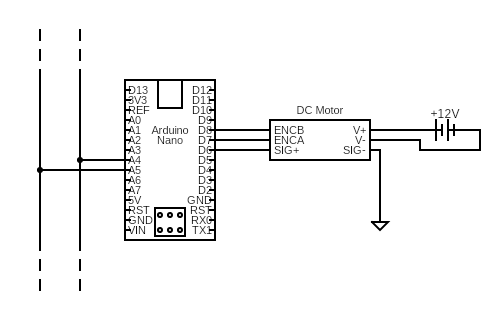
\includegraphics[width=\maxwidth{\textwidth}]{img/slave-schematics}
  \caption{Slave controller schematics}
  \label{img:slave-sch}
\end{centering}
\end{figure}

\subsection{Wiring}
The wiring correspondence for the slave controller MCU is shown in table
\ref{tab:slave-wiring}.
\begin{table}[hb]
  \begin{tabularx}{\textwidth}{c l X}
    \toprule
    Board pin & MCU pin & Description \\
    \midrule
    A4 & 27/PC4/ADC4/SDA  & I2C data bus \\
    A5 & 28/PC5/ADC5/SCL  & I2C clock bus \\
    D6 & 10/PD6/AIN0/OC0A & PWM output to the dc motor \\
    D7 & 11/PD7/AIN1/ICP1 & Encoder phase A, interrupt-enabled \\
    D8 & 12/PB0/CLK0      & Encoder phase B \\
    \bottomrule
  \end{tabularx}
  \caption{Slave controller wiring}
  \label{tab:slave-wiring}
\end{table}


\chapter{Client-Master communication}
\label{ch:client-master-comm}
The client application and the master controller communicate over a protocol
built on top of the serial-over-usb layer. Such protocol is completely binary
and packet-based. Each packet has a variable length (with a total maximum size
of 36 bytes) and its integrity is checked with a trailing CRC-8 checksum.

The protocol comes with a simple handshaking mechanism, in order to synchronize
the packet IDs between endpoints and as a shallow proof of correct
functionality of the communication layers.

\section{Serial layer}
Data exchange between client and master relies on the serial protocol. For the
client application, the \emph{termios} library is used, while for the master
controller the (hardware) serial subsystem offered by the AVR
microcontroller\cite{at2560-ref} is used.

The serial communication is set up as follows:
\begin{itemize}
  \item Baud rate of 115200 baud, double speed transmission
  \item 8 bit frame width
  \item No start bits, 1 stop bit (i.e.\ 8N1)
  \item No embedded parity bit
\end{itemize}

For the master controller, both transmission and reception are
interrupt-driven, so the communication main routine is only called when data is
actually available.

\section{Packet headers}
Each packet's metadata is contained in a fixed size header, composed as
describe in table \ref{tab:packet-header}.

\begin{table}[bh]
  \begin{tabularx}{\textwidth}{c c X}
    \toprule
    Field & Size (bits) & Description \\
    \midrule
    id       & $8$ & Packet ID \\
    type     & $8$ & Packet type \\
    selector & $8$ & Selector for DC motors. Also used to store error codes in NAK packets \\
    size     & $8$ & Total packet size, including header and checksum \\
    \bottomrule
  \end{tabularx}
  \caption{Packet header fields}
  \label{tab:packet-header}
\end{table}

\subsection{Identifiers}
The \emph{id} field stores the packet identifier, which is incremental and can
be repeated in a single communication session. When the handshake is performed,
or when any endpoint raises an error (issuing a \emph{NAK} packet), the id is
reset to zero for both sides. Each \emph{ACK} and \emph{NAK} packet is
generated with the same id of the referred packet (see
\ref{client-master-comm-ackerr} for further informations).

\subsection{Packet types}
The \emph{type} field stores the packet type. An exhaustive list of packet
types is given in table \ref{tab:packet-types}

\begin{table}[bh]
  \begin{tabularx}{\textwidth}{c c X}
    \toprule
    Type & Code & Description \\
    \midrule
    \texttt{NULL}       & \texttt{0x00} & Reserved, never use \\
    \texttt{HND}        & \texttt{0x01} & Handshake \\
    \texttt{ACK}        & \texttt{0x02} & Acknowledgement \\
    \texttt{NAK}        & \texttt{0x03} & Communication error \\
    \texttt{ECHO}       & \texttt{0x04} & Echo between Client and Master (debug only)\\
    \texttt{TWI\_ECHO}  & \texttt{0x05} & Echo a single char to the first Slave via TWI (debug only)\\
    \texttt{GET\_SPEED} & \texttt{0x06} & Get the current speed for a DC motor \\
    \texttt{SET\_SPEED} & \texttt{0x07} & Set (and apply) the speed for a DC motor \\
    \texttt{APPLY}      & \texttt{0x08} & Tell all the slaves to apply the previously set speeds \\
    \texttt{DAT}        & \texttt{0x09} & Primarily used for responses from the AVR device \\
    \texttt{LIMIT}      & \texttt{0x0A} & Used for sanity checks - Must have highest value \\
    \bottomrule
  \end{tabularx}
  \caption{Exhaustive list of packet types}
  \label{tab:packet-types}
\end{table}

\subsection{Motor selector}
The \emph{selector} field is used to store the identifier for the dc motor to
manipulate. This field is used in \texttt{GET\_SPEED} and \texttt{SET\_SPEED} packets.

For \emph{NAK} packets, instead, the \emph{selector} field is used to store
error codes (found in table \ref{tab:packet-error-codes}).

For all the other packet types, the \emph{selector} field is ignored.

\section{Acknowledgements and errors}
\label{client-master-comm-ackerr}
A communication endpoint must wait for an acknowledgement message from the
counterpart once it sent a packet in order to send a new one. ACK and NAK
packets do not bring any data.

When a packet arrives, it is checked for integrity and sanity. If it is sane,
then an ACK packet is sent; if not, then a NAK packet is sent.
ACK and NAK packets are simply discarded if corrupted in some way.

A NAK packet uses the \emph{selector} field to send to the other endpoint the
error code describing what happened on its side. Error codes are listed in
table \ref{tab:packet-error-codes}.

\begin{table}[bh]
  \begin{tabularx}{\textwidth}{c c X}
    \toprule
    Error & Code & Description \\
    \midrule
    \texttt{SUCCESS}             & \texttt{0x00} & No errors encountered \\
    \texttt{ID\_MISMATCH}        & \texttt{0x01} & Id of received packet is not consistent \\
    \texttt{CORRUPTED\_CHECKSUM} & \texttt{0x02} & Checksum mismatch, received packet is corrupted \\
    \texttt{WRONG\_TYPE}         & \texttt{0x03} & Received packet has invalid type \\
    \texttt{TOO\_BIG}            & \texttt{0x04} & Received packet has invalid size (too big) \\
    \bottomrule
  \end{tabularx}
  \caption{Exhaustive list of packet types}
  \label{tab:packet-error-codes}
\end{table}


\chapter{Master-Slave communication}
\label{ch:master-slave-comm}
The master and slave controllers communicate to each other using the I2C
bus. Naturally, the master controller is responsible for starting communication
sessions, addressing one or all the slaves.

The bitrate is set to 100kbit/s, i.e.\ the maximum speed available for the
original I2C standard\cite{i2c-ref} (excluding fast modes, which were
implemented later).

\subsection{Hardware setup}
The I2C bus itself is a pair of bus rails, named \texttt{SDA} and \texttt{SCL},
representing data and bus clock respectively.

Two $4.7 k\Omega$ resistors connects SDA and SCL to a $5V$ voltage generator
and act as \emph{open-drain} resistors.
% TODO: Footnote?

\subsection{Communication frames}
The first byte of the I2C communication frame (excluding, of course, the slave
address) is an 8-bit unsigned integer representing the command sent by the
master to the slave. The trailing data represents an argument, with its size
and shape depending on the type of command issued. Command codes, with their
specific arguments, are shown in table \ref{tab:i2c-commands}.

\begin{table}[bh]
  \begin{tabularx}{\textwidth}{c c c X}
    \toprule
    Command & Code & Argument size (bytes) & Description \\
    \midrule
      \texttt{DC\_MOTOR\_CMD\_GET}   & \texttt{0x00} & - & Get the dc motor speed in rpm \\
      \texttt{DC\_MOTOR\_CMD\_SET}   & \texttt{0x01} & 1 & Set the dc motor target speed \\
      \texttt{DC\_MOTOR\_CMD\_APPLY} & \texttt{0x02} & - & Apply the previously set target speed \\
      \texttt{TWI\_CMD\_ECHO}        & \texttt{0x03} & 1 & Send back the received character to the master (debug)\\
    \bottomrule
  \end{tabularx}
  \caption{Master-to-slave commands}
  \label{tab:i2c-commands}
\end{table}


\chapter{Conclusions}
\label{ch:conclusions}


\backmatter
\cleardoublepage
\phantomsection % Give this command only if hyperref is loaded

\addcontentsline{toc}{chapter}{\bibname}
\bibliographystyle{plain}
\bibliography{main}

\end{document}
